\chapter{Expectation}

\begin{ex}
  Let $X_i$ take on the values $\left\{\frac{1}{2}, 2\right\}$ depending on
  whether the $i$th turn of the game resulted in a halving or a doubling
  respectively. Since both outcomes occur with equal probability,
  \[
    \E{X_i} = \frac{1}{2}\cdot \frac{1}{2} + 2\cdot \frac{1}{2}=\frac{5}{4}.
  \]

  Let $Y_n$ be the amount of money we have after the $n$th turn, and note that
  \[
    Y_n = c\prod_{i=1}^nX_i,
  \]
  where $X_i$ is independent of $X_j$ whenever $i\neq j$. Therefore,
  \begin{align*}
    \E{Y_n}
    =\E{c\prod_{i=1}^nX_i}
    =c\prod_{i=1}^n\E{X_i}
    =c\left(\frac{5}{4} \right)^{n}.
  \end{align*}
\end{ex}

\begin{ex}
  Suppose that there is a constant $c$ such that $\P{X=c}=1$. It follows that
  $X$ is a discrete random variable, and therefore
  \[
    \E{X}=\sum_{x\in \supp(X)} x\P{X=x}=c,
  \]
  since $\P{X=x}=0$ for $x\neq c$. Likewise,
  \[
    \E{X^2}=\sum_{x\in \supp(X)} x^2\P{X=x}=c^2,
  \]
  and so
  \[
    \var{X}=\E{X^2}-\E{X}^2=c^2-c^2=0.
  \]

  For the converse, we begin by proving a lemma. Let $Y$ be a non-negative
  random variable such that $\E{Y}=0$. We want to prove that $\P{Y=0}=1$.

  Let $B_n=[1/n,\infty)$ and note that
  \[
    0=\E{Y}\geq \frac{1}{n}\P{X\in B_n},
  \]
  and hence $\P{B_n}=0$. However,
  \[
    1 = \P{X\in \{0\}\cup\bigcup_{n=1}^\infty B_n}=\P{X=0}+\lim_{n\to\infty}
    \P{X\in B_m}= \P{X=0}.
  \]

  For the converse of the original claim, suppose we are given a random variable
  $X$ such that $\var{X}=0$. Note that we assume that $X$ has a mean in our
  definition of variance, and therefore can let $\E{X}=c$. Hence,
  \[
    \E{(X-c)^2}=0,
  \]
  or, by our previous lemma,
  \[
    \P{(X-c)^2= 0}=1.
  \]
  But this is equivalent to $\P{X=c}=1$.
\end{ex}

\begin{ex}
  Let $X_1,\ldots,X_n\sim\text{Uniform}(0, 1)$ and let
  $Y_n=\max\{X_1,\ldots,X_n\}$. Then
  \[
    \P{Y_n\leq y}y
    =\P{X_1\leq y}\cdots \P{X_n\leq y}
    =\begin{cases}
      0   & y<0,          \\
      y^n & 0\leq y\leq1, \\
      1   & y>1,
    \end{cases}
  \]
  and therefore
  \[
    f_{Y_n}(y)=\begin{cases}
      ny^{n-1} & 0\leq y\leq1      \\
      0        & \text{otherwise}.
    \end{cases}
  \]

  Hence,
  \[
    \E{Y_n}
    =\int_0^1\! ny^n\,\d{y}
    =\frac{n y^{n+1}}{n+1}\,\bigg\rvert_{y=0}^1
    =\frac{n}{n+1}.
  \]
\end{ex}

\begin{ex}
  Let $J_i$ be the outcome of the $i$th jump: $-1$ if it is a jump to the left
  and $1$ if it is a jump to the right. Note that
  \begin{align*}
    \E{J_i}   & =-1\cdot p+1\cdot (1-p)=1-2p,        \\
    \E{J_i^2} & =1\cdot p+1\cdot (1-p)=1\text{, and} \\
    \var{J_i} & =1-(1-2p)^2=4p-4p^2.
  \end{align*}

  Let $X_n$ be the position of the particle after $n$ time units. Note that
  $X_n=\sum_{i=1}^n J_i$, where all the $J_i$'s are independent. Therefore,
  \[
    \E{X_n}
    = \E{\sum_{i=1}^n J_i}
    = \sum_{i=1}^n \E{J_i}
    = n(1-2p) \text{, and}
  \]
  \[
    \var{X_n}
    = \var{\sum_{i=1}^n J_i}
    = \sum_{i=1}^n \var{J_i}
    = n(4p-4p^2).
  \]
\end{ex}

% 5
\begin{ex}
  Let $X$ be the number of fair coin tosses until a head is obtained. Note that
  since the only way to obtain the first head in $n$ tosses is to toss tails
  $n-1$ times and then toss a head, it follows that
  $\P{X=n}=\left(\frac{1}{2}\right)^n$.
  Hence,
  \[
    \E{X}
    = \sum_{n=1}^\infty n\cdot \left(\frac{1}{2}\right)^n
    = 2
  \]
  by comparison to the Taylor series of $x/(1-x)^2$.
\end{ex}

\begin{ex}
  Note that
  \[
    \E{r(X)}
    =\sum_{y\in\supp{Y}}y\P{r(X)=y}
    =\sum_{y\in\supp{Y}}y\sum_{\{x\in\supp{X}\mid r(x)=y\}}\P{X=x},
  \]
  where the double summation $\sum_y\sum_{\{x\mid r(x)=y\}}$ is equivalent to
  the single summation $\sum_{x}$ by replacing $y$ with $r(x)$. Hence,
  \[
    \E{r(X)}
    =\sum_{x\in\supp{X}}r(x)f_X(x).
  \]
\end{ex}

\begin{ex}
  Let $X$ be a continuous random variable with CDF $F$, such that $\P{X>0}=1$
  and $\E{X}$ exists. Note that then $\P{X\leq 0}=1-\P{X>0}=0$. Then
  \begin{align*}
    \int_{0}^\infty\! \P{X>x}\,\d{x}
     & =\int_{0}^\infty\! 1-F(x)\,\d{x}                                                                                \\
     & =x(1-F(x))\,\bigg\rvert_{x=0}^\infty+\int_{0}^\infty\! xF'(x)\,\d{x} &  & (\text{integration by parts})         \\
     & =\int_{0}^\infty\! xF'(x)\,\d{x}                                                                                \\
     & =\int_{-\infty}^\infty\! xF'(x)\,\d{x}                               &  & (\text{since $F(x)=0$ for $x\leq 0$}) \\
     & =\E{X}.
  \end{align*}

\end{ex}

\begin{ex}
  Let $X_1,\ldots,X_n$ be \iid with $\mu=\E{X_i}$ and $\sigma^2=\var{X_i}$. Then
  \begin{align*}
    \E{\overline{X}_n}
     & =\E{\frac{\sum_{i=1}^nX_i}{n}}                                      \\
     & =\frac{1}{n}\sum_{i=1}^n\E{X_i} & \text{(linearity of expectation)} \\
     & =\frac{n\mu}{n}                                                     \\
     & =\mu.
  \end{align*}

  Likewise,
  \begin{align*}
    \var{\overline{X}^2_n}
     & =\var{\frac{\sum_{i=1}^nX_i}{n}}           \\
     & =\frac{1}{n^2}\sum_{i=1}^n\var{X_i}        \\
     & =\frac{n\sigma^2}{n^2}=\frac{\sigma^2}{n}.
  \end{align*}

  Finally, observe that
  \[
    \E{X_i^2}
    =\var{X_i}+\E{X_i}^2
    =\sigma^2+\mu^2,
  \]
  \[
    \E{\overline{X}^2_n}
    =\var{\overline{X}_n}+\E{\overline{X}_n}^2
    =\frac{\sigma^2}{n}+\mu^2,
  \]
  and
  \begin{align*}
    \E{X_i\overline{X}_n}
     & =\frac{1}{n}\E{X_i\sum_{j=1}^nX_j}                                           \\
     & =\frac{1}{n}\E{X^2_i+\sum_{\substack{j=1                                     \\ j\neq i}}^n X_iX_j} \\
     & =\frac{1}{n}\left(\sigma^2+\mu^2+(n-1)\mu^2\right)=\frac{\sigma^2}{n}+\mu^2,
  \end{align*}
  and that therefore
  \begin{align*}
    \E{S^2_n}
     & =\E{\frac{1}{n-1}\sum_{i=1}^n\left(X_i-\overline{X}_n)^2\right)}                               \\
     & =\frac{1}{n-1}\sum_{i=1}^n\E{\left(X_i-\overline{X}_n)^2\right)}                               \\
     & =\frac{1}{n-1}\sum_{i=1}^n\E{X_i^2-2X_i\overline{X_n}+\overline{X}_n^2}                        \\
     & =\frac{n}{n-1}\left(\sigma^2+\mu^2-\frac{2\sigma^2}{n}-2\mu^2+\frac{\sigma^2}{n}+\mu^2 \right) \\
     & =\frac{n}{n-1}\left(\sigma^2-\frac{\sigma^2}{n}\right)                                         \\
     & =\sigma^2.
  \end{align*}
\end{ex}

\begin{ex}
  We use the following Python code to graph the sample means:

  \inputminted{python}{src/03-09a.py}

  \begin{figure}[H]
    \centering
    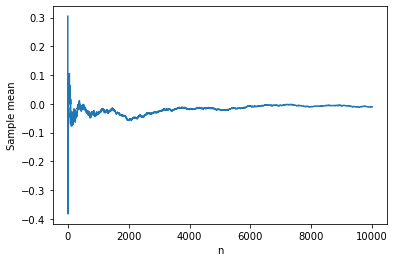
\includegraphics[scale=0.9]{part1/ch03-09a}
    \caption{Graph of $\overline{X}_n$ for a standard normal distribution.}
  \end{figure}

  \inputminted{python}{src/03-09b.py}

  \begin{figure}[H]
    \centering
    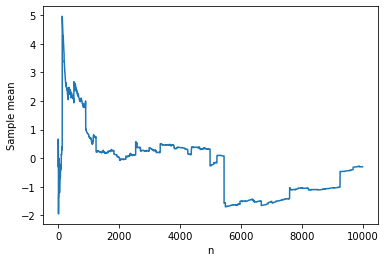
\includegraphics[scale=0.9]{part1/ch03-09b}
    \caption{Graph of $\overline{X}_n$ for a Cauchy distribution.}
  \end{figure}

  The standard normal distribution has a defined mean of $0$ and, as expected,
  the sample mean seems to be converging to it. The Cauchy distribution does not
  have a mean, and that is why the sample mean is not converging to a particular
  value.
\end{ex}

% 10
\begin{ex}
  Let $X\sim N(0, 1)$ and let $Y=e^X$. Then
  \begin{align*}
    \E{Y}
     & =\int_{-\infty}^\infty\!\frac{e^x}{\sqrt{2\pi}}e^{-\frac{1}{2}x^2}\,\d{x}                    \\
     & =\int_{-\infty}^\infty\!\frac{1}{\sqrt{2\pi}}e^{-\frac{1}{2}(x^2-2x)}\,\d{x}                 \\
     & =\int_{-\infty}^\infty\!\frac{e^{\frac{1}{2}}}{\sqrt{2\pi}}e^{-\frac{1}{2}(x^2-2x+1)}\,\d{x} \\
     & =e^{\frac{1}{2}}\int_{-\infty}^\infty\!\frac{1}{\sqrt{2\pi}}e^{-\frac{1}{2}(x-1)^2}\,\d{x}   \\
     & =e^{\frac{1}{2}}.
  \end{align*}

  Recall that $\var{Y}=\E{Y^2}-\E{Y}^2$, and note that
  \begin{align*}
    \E{Y^2}
     & =\int_{-\infty}^\infty\!\frac{e^{2x}}{\sqrt{2\pi}}e^{-\frac{1}{2}x^2}\,\d{x}     \\
     & =\int_{-\infty}^\infty\!\frac{1}{\sqrt{2\pi}}e^{-\frac{1}{2}(x^2-4x)}\,\d{x}     \\
     & =\int_{-\infty}^\infty\!\frac{e^2}{\sqrt{2\pi}}e^{-\frac{1}{2}(x^2-4x+4)}\,\d{x} \\
     & =e^2\int_{-\infty}^\infty\!\frac{1}{\sqrt{2\pi}}e^{-\frac{1}{2}(x-2)^2}\,\d{x}   \\
     & =e^2.
  \end{align*}
  Therefore,
  \[
    \var{Y}=e^2-e.
  \]
\end{ex}

\begin{ex}
  \begin{enumerate}[(a)]
    \item Note that $X_n$ is identical to the $X_n$ of Exercise 3.4 with
          $p=\frac{1}{2}$. Therefore, $\E{X_n}=0$ and $\var{X_n}=n$.
    \item We use the following Python code.
          \inputminted{python}{src/03-11.py}

          \begin{figure}[H]
            \centering
            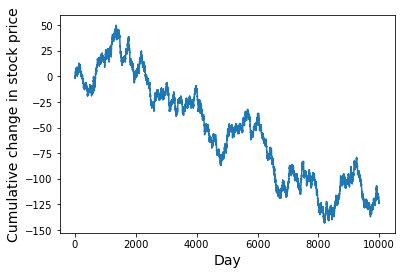
\includegraphics[scale=0.8]{part1/ch03-11a}
            \caption{First simulation of $X_n$.}
          \end{figure}

          \begin{figure}[H]
            \centering
            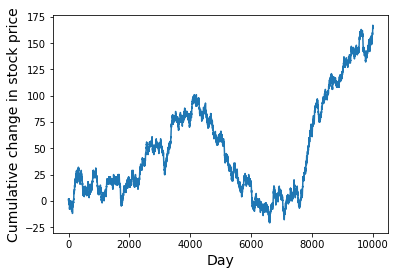
\includegraphics[scale=0.8]{part1/ch03-11b}
            \caption{Second simulation of $X_n$.}
          \end{figure}

          \begin{figure}[H]
            \centering
            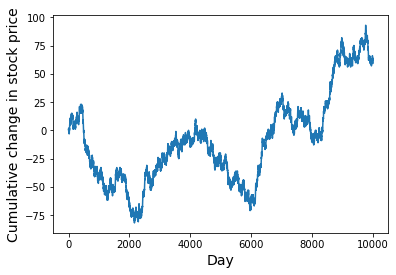
\includegraphics[scale=0.8]{part1/ch03-11c}
            \caption{Third simulation of $X_n$.}
          \end{figure}

          The expected value of $X_n$ is $0$, but none of the simulations show
          $X_n$ converging to $0$. This is explainable by the fact that the
          variance is increasing with $n$.
  \end{enumerate}
\end{ex}

\begin{ex}
  % Bernoulli
  Let $B$ be a $\text{Bernoulli}(p)$ random variable. Then
  \begin{align*}
    \E{B}   & =(1-p)\cdot 0 + p\cdot 1 = p,     \\
    \E{B^2} & =(1-p)\cdot 0^2 + p\cdot 1^2 = p, \\
    \var{B} & = \E{B^2}-\E{B}^2=p-p^2=p(1-p).
  \end{align*}

  % Poisson
  Let $P$ be a $\text{Poisson}(\lambda)$ random variable. Then
  \begin{align*}
    \E{P}
     & =\sum_{k=1}^\infty k\frac{e^{-\lambda}\lambda^{k}}{k!}              \\
     & =e^{-\lambda}\lambda \sum_{k=1}^\infty \frac{\lambda^{k-1}}{(k-1)!} \\
     & =e^{-\lambda}\lambda \sum_{k=0}^\infty \frac{\lambda^{k}}{k!}       \\
     & = \lambda,
  \end{align*}
  \begin{align*}
    \E{P^2}
     & =\sum_{k=1}^\infty k^2\frac{e^{-\lambda}\lambda^{k}}{k!}                                                        \\
     & =e^{-\lambda}\lambda\sum_{k=1}^\infty k\frac{\lambda^{k-1}}{(k-1)!}                                             \\
     & =e^{-\lambda}\lambda\sum_{k=0}^\infty (k+1)\frac{\lambda^k}{k!}                                                 \\
     & =e^{-\lambda}\lambda\left[\sum_{k=0}^\infty k\frac{\lambda^k}{k!}+\sum_{k=0}^\infty \frac{\lambda^k}{k!}\right] \\
     & =e^{-\lambda}\lambda\left[\lambda e^{\lambda} + e^{\lambda}\right]                                              \\
     & =\lambda^2+\lambda,
  \end{align*}
  and therefore
  \[
    \var{P}
    =\E{P^2}-\E{P}^2
    =\lambda^2+\lambda-\lambda=\lambda.
  \]

  % Uniform
  Let $U$ be a $\text{Uniform}(a, b)$ random variable. Then
  \begin{align*}
    \E{U}   & = \int_a^b\!\frac{x}{b - a}\,\d{x}
    =\frac{1}{2}\frac{b^2-a^2}{b-a}
    =\frac{a + b}{2},                              \\
    \E{U^2} & = \int_a^b\!\frac{x^2}{b - a}\,\d{x}
    =\frac{1}{3}\frac{b^3-a^3}{b-a}
    =\frac{a^2+ab+b^2}{3},\text{ and hence}        \\
    \var{U} & = \E{U^2}-\E{U}^2
    =\frac{a^2+ab+b^2}{3}-\frac{a^2+2ab+b^2}{4}
    =\frac{(b-a)^2}{12}.
  \end{align*}

  % Exponential
  Let $X$ be an $\text{Exponential}(\beta)$ random variable. Then
  \begin{align*}
    \E{X}
     & =\int_0^\infty\!\frac{x}{\beta}e^{-x/\beta}\,\d{x}                                            \\
     & =\beta\int_0^\infty\!ue^{-u}\,\d{u}                                             & (u=x/\beta) \\
     & =\beta\left[-ue^{-u}\bigg\rvert_{u=0}^\infty-\int_0^\infty e^{-u}\,\d{u}\right]               \\
     & =\beta,
  \end{align*}
  \begin{align*}
    \E{X^2}
     & =\int_0^\infty\!\frac{x^2}{\beta}e^{-x/\beta}\,\d{x}                                  \\
     & =\beta^2\int_0^\infty\!u^2e^{-u}\,\d{u}                                               \\
     & =\beta^2\left[u^2e^{-u}\bigg\rvert_{u=0}^\infty-2\int_0^\infty ue^{-u}\,\d{u} \right] \\
     & =2\beta^2,
  \end{align*}
  and hence
  \[
    \var{X}
    =\E{X^2}-\E{X}^2
    =2\beta^2-\beta^2=\beta^2.
  \]

  % Gamma
  Let $G$ be an $\text{Gamma}(\alpha, \beta)$ random variable. Then
  \begin{align*}
    \E{G}
     & =\int_0^\infty\!\frac{x}{\beta^\alpha\Gamma(\alpha)}x^{\alpha-1}e^{-x/\beta}\,\d{x}                                                 \\
     & =\frac{\beta\Gamma(\alpha+1)}{\Gamma(\alpha)}\int_0^\infty\!\frac{1}{\beta^{\alpha+1}\Gamma(\alpha+1)}x^{\alpha}e^{-x/\beta}\,\d{x} \\
     & =\alpha\beta,
  \end{align*}
  \begin{align*}
    \E{G^2}
     & =\int_0^\infty\!\frac{x^2}{\beta^\alpha\Gamma(\alpha)}x^{\alpha-1}e^{-x/\beta}\,\d{x}                                                   \\
     & =\frac{\beta^2\Gamma(\alpha+2)}{\Gamma(\alpha)}\int_0^\infty\!\frac{1}{\beta^{\alpha+2}\Gamma(\alpha+2)}x^{\alpha+1}e^{-x/\beta}\,\d{x} \\
     & =\alpha(\alpha+1)\beta^2,
  \end{align*}
  and thus
  \[
    \var{G}
    =\E{G^2}-\E{G}^2
    =\alpha(\alpha+1)\beta^2-\alpha^2\beta^2
    =\alpha\beta^2.
  \]

  % Beta
  Finally, let $Y$ be a $\text{Beta}(\alpha, \beta)$ random variable. Then
  \begin{align*}
    \E{Y}
     & =\int_0^\infty\!x\cdot\frac{\Gamma(\alpha+\beta)}{\Gamma(\alpha)\Gamma(\beta)}x^{\alpha-1}(1-x)^{\beta-1} \,\d{x}                                                                             \\
     & =\frac{\Gamma(\alpha+\beta)\Gamma(\alpha+1)}{\Gamma(\alpha)\Gamma(\alpha+\beta+1)}\int_0^\infty\!\frac{\Gamma(\alpha+\beta+1)}{\Gamma(\alpha+1)\Gamma(\beta)}x^{\alpha}(1-x)^{\beta-1}\,\d{x} \\
     & =\frac{\alpha}{\alpha+\beta},
  \end{align*}
  \begin{align*}
    \E{Y^2}
     & =\int_0^\infty\!x^2\cdot\frac{\Gamma(\alpha+\beta)}{\Gamma(\alpha)\Gamma(\beta)}x^{\alpha-1}(1-x)^{\beta-1} \,\d{x}                                                                             \\
     & =\frac{\Gamma(\alpha+\beta)\Gamma(\alpha+2)}{\Gamma(\alpha)\Gamma(\alpha+\beta+2)}\int_0^\infty\!\frac{\Gamma(\alpha+\beta+2)}{\Gamma(\alpha+2)\Gamma(\beta)}x^{\alpha+1}(1-x)^{\beta-1}\,\d{x} \\
     & =\frac{\alpha(\alpha+1)}{(\alpha+\beta+1)(\alpha+\beta)},
  \end{align*}
  and so
  \begin{align*}
    \var{Y}
     & =\E{Y^2}-\E{Y}^2                                         \\
     & =\frac{\alpha(\alpha+1)}{(\alpha+\beta+1)(\alpha+\beta)}
    -\frac{\alpha^2}{(\alpha+\beta)^2}                          \\
     & =\frac{\alpha\beta}{(a+\beta)^2(\alpha+\beta+1)}.
  \end{align*}
\end{ex}

\begin{ex}
  Let $Z$ be a uniform discrete random variable on $\{0, 1\}$,
  $X_1\sim\text{Uniform}(0, 1)$ and $X_2\sim\text{Uniform}(3, 4)$. Then
  $X=ZX_1 + (1-Z)X_2$.
  \begin{itemize}[(a)]
    \item We have
          \begin{align*}
            \E{X} & =\E{ZX_1 + (1-Z)X_2}           \\
                  & =\E{ZX_1} + \E{(1-Z)X_2}       \\
                  & =\E{Z}\E{X_1} + \E{1-Z}\E{X_2} \\
                  & =\frac{1}{4}+\frac{7}{4}       \\
                  & =2.
          \end{align*}
    \item[(b)] We begin by finding the variance:
          \begin{align*}
            \var{X}
             & =\var{ZX_1 + (1-Z)X_2}                           \\
             & =\var{ZX_1}+\var{(1-Z)X_2}+2\cov{ZX_1, (1-Z)X_2} \\
             & =\frac{5}{48}+\frac{149}{48}-\frac{7}{8}         \\
             & =\frac{7}{3},
          \end{align*}
          since
          \begin{align*}
            \var{ZX_1}
             & =\E{Z^2}\E{X_1^2}-\frac{1}{16}
            =\frac{1}{2}\cdot\frac{1}{3}-\frac{1}{16}
            =\frac{5}{48},                            \\
            \var{(1-Z)X_2}
             & =\E{(1-Z)^2}\E{X_2^2}-\frac{49}{16}
            =\frac{1}{2}\cdot\frac{37}{3}-\frac{49}{16}
            =\frac{149}{48},\text{ and}               \\
            \cov{ZX_1, (1-Z)X_2}
             & =\E{Z(1-Z)X_1X_2}-\E{ZX_1}\E{(1-Z)X_2}
            =-\frac{1}{4}\cdot\frac{7}{4}
            =-\frac{7}{16}.
          \end{align*}
          Therefore, the standard deviation is $\sqrt{7/3}$.
  \end{itemize}
\end{ex}

\begin{ex}
  Let $X_1,\ldots, X_m$ and $Y_1,\ldots,Y_n$ be random variables and
  $a_1,\ldots,a_m,b_1,\ldots,b_n$ be constants. Then
  \begin{align*}
    \cov{\sum_{i=1}^m a_iX_i, \sum_{j=1}^nb_jY_j }
     & =\E{\left(\sum_{i=1}^m a_iX_i\right)\left(\sum_{j=1}^nb_jY_j\right)}
    -\E{\sum_{i=1}^m a_iX_i}\E{\sum_{j=1}^nb_jY_j}                             \\
     & =\E{\sum_{i=1}^m \sum_{j=1}^n a_ib_jX_iY_j}
    -\left[\sum_{i=1}^m a_i\E{X_i}\right] \left[\sum_{j=1}^n b_j\E{Y_j}\right] \\
     & =\sum_{i=1}^m\sum_{j=1}^n a_ib_j \E{X_iY_j}
    -\sum_{i=1}^m\sum_{j=1}^n a_ib_j \E{X_i}\E{Y_j}                            \\
     & =\sum_{i=1}^m\sum_{j=1}^n a_ib_j\left[\E{X_iY_j}-\E{X_i}\E{Y_j}\right]  \\
     & =\sum_{i=1}^m\sum_{j=1}^n a_ib_j\cov{X_i, Y_j}.
  \end{align*}
\end{ex}

% 15
\begin{ex}
  Let $X,Y$ be random variables with joint PDF
  \[
    f_{X, Y}(x,y)
    =\begin{cases}
      \frac{1}{3}\left(x+y\right) & 0\leq x\leq 1, 0\leq y\leq 2 \\
      0                           & \text{otherwise}.
    \end{cases}
  \]

  Note that
  \begin{align*}
    f_X(x)
     & =\int_0^2\! f_{X,Y}(x,y)\,\d{y}                      \\
     & =\int_0^2\! \frac{1}{3}x+\frac{1}{3}y\,\d{y}         \\
     & =\left[ \frac{1}{3}xy+\frac{1}{6}y^2 \right]_{y=0}^2 \\
     & =\frac{2}{3}\left(x+1\right),
  \end{align*}
  and that therefore
  \[
    \E{X}
    =\int_0^1\!x\cdot\frac{2}{3}\left(x+1\right)\,\d{x}
    =\left[ \frac{2}{9}x^3+\frac{1}{3}x^2 \right]_{x=0}^1
    =\frac{5}{9},
  \]
  \[
    \E{X^2}
    =\int_0^1\!x^2\cdot\frac{2}{3}\left(x+1\right)\,\d{x}
    =\left[ \frac{2}{12}x^4+\frac{2}{9}x^3 \right]_{x=0}^1
    =\frac{7}{18},
  \]
  and
  \begin{align*}
    \var{X}=\E{X^2}-\E{X}^2=\frac{7}{18}-\frac{25}{81}=\frac{13}{162}.
  \end{align*}

  Similarly,
  \begin{align*}
    f_Y(y)
     & =\int_0^1\! f_{X,Y}(x,y)\,\d{x}                    \\
     & =\int_0^1\! \frac{1}{3}x+\frac{1}{3}y\,\d{x}       \\
     & =\left[\frac{1}{6}x^2+\frac{1}{3}xy\right]_{x=0}^1 \\
     & =\frac{1}{6}+\frac{1}{3}y,
  \end{align*}
  and so
  \begin{align*}
    \E{Y}
    =\int_0^2\!y\left(\frac{1}{6}+\frac{1}{3}y\right)\,\d{y}
    =\left[ \frac{1}{12}y^2+\frac{1}{9}y^3 \right]_{y=0}^2
    =\frac{11}{9},
  \end{align*}
  \begin{align*}
    \E{Y^2}
    =\int_0^2\!y^2\left(\frac{1}{6}+\frac{1}{3}y\right)\,\d{y}
    =\left[ \frac{1}{18}y^3+\frac{1}{12}y^4 \right]_{y=0}^2
    =\frac{16}{9},
  \end{align*}
  and
  \begin{align*}
    \var{Y}=\E{Y^2}-\E{Y}^2=\frac{16}{9}-\frac{121}{81}=\frac{23}{81}.
  \end{align*}

  Note that
  \begin{align*}
    \E{XY}
    =\int_0^2\!\int_0^1\!\frac{1}{3}x^2y+\frac{1}{3}xy^2\,\d{x}\,\d{y}
    =\int_0^2\!\frac{1}{6}y^2+\frac{1}{9}y\,\d{y}
    =\frac{2}{3},
  \end{align*}
  and so
  \begin{align*}
    \cov{X,Y}=\E{XY}-\E{X}\E{Y}=\frac{2}{3} - \frac{55}{81}=-\frac{1}{81}.
  \end{align*}

  Therefore,
  \begin{align*}
    \var{2X-3Y+8}
    =4\var{X}+9\var{Y}-12\cov{X,Y}
    =\frac{26}{81}+\frac{207}{81} +\frac{12}{81}
    =\frac{245}{81}.
  \end{align*}

\end{ex}

\begin{ex}
  We will assume that $X$ and $Y$ are continuous random variables and note that
  the proof in the discrete case proceeds similarly. Then
  \begin{align*}
    \cE{r(X)s(Y)}{X=x}
     & =\int_\R\!r(x)s(y)f_{X|Y}(x|y)\,\d{y} \\
     & =r(x)\int_\R\!s(y)f_{X|Y}(x|y)\,\d{y} \\
     & =r(x)\cE{s(y)}{X=x},
  \end{align*}
  and we note that if we let $g(y)=1$,
  \[
    \cE{r(X)s(Y)}{X=x}
    =\cE{r(X)}{X=x}
    =r(x)\cE{1}{X=x}=r(x).
  \]
\end{ex}

\begin{ex}
  We have
  \begin{align*}
    \var{Y}
     & =\E{Y^2}-\E{Y}^2                                   \\
     & =\E{\cE{Y^2}{X}}-\E{\cE{Y}{X}}^2                   \\
     & =\E{\var{Y\,|\,X}}+\E{\cE{Y^2}{X}}-\E{\cE{Y}{X}}^2 \\
     & =\E{\var{Y\,|\,X}}+\E{\cE{Y^2}{X}-\cE{Y}{X}^2}     \\
     & =\E{\var{Y\,|\,X}}+\var{\cE{Y}{X}}.
  \end{align*}
\end{ex}

\begin{ex}
  Note that
  \[
    \E{XY}
    =\E{\cE{XY}{Y}}
    =\E{Y\cE{X}{Y}}
    =c\E{Y},
  \]
  \[
    \E{X}
    =\E{\cE{X}{Y}}
    =c,
  \]
  and that therefore
  \[
    \cov{X,Y}
    =\E{XY}-\E{X}\E{Y}
    =c\E{Y}-c\E{Y}
    =0.
  \]
\end{ex}

\begin{ex}
  Note that $f_X(x)=I_{[0,1]}(x)$.
  \begin{figure}[H]
    \centering
    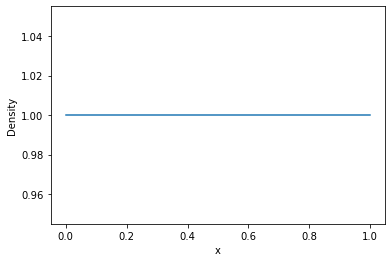
\includegraphics[scale=0.8]{part1/ch03-19a}
    \caption{Graph of $f_X$.}
  \end{figure}

  We have
  \[
    \E{\overline{X}_n}
    =\E{\frac{1}{n}\sum_{i=1}^n X_i}
    =\E{X_1}=\frac{1}{2}, \text{ and}
  \]
  \[
    \var{\overline{X}_n}
    =\frac{n}{n^2}\var{X_1}
    =\frac{1}{12n}.
  \]

  \inputminted{python}{src/03-19b.py}

  \begin{figure}[H]
    \centering
    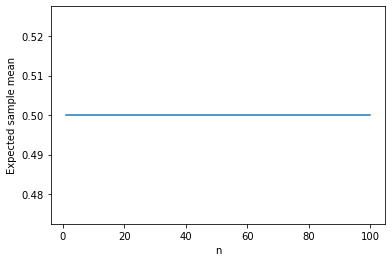
\includegraphics[scale=0.8]{part1/ch03-19b}
    \caption{Graph of $\E{\overline{X}_n}$ as a function of $n$.}
  \end{figure}

  \inputminted{python}{src/03-19c.py}

  \begin{figure}[H]
    \centering
    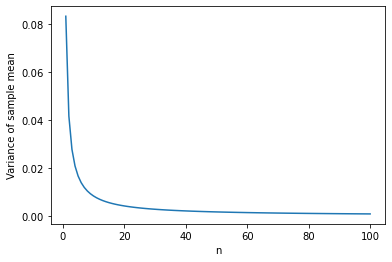
\includegraphics[scale=0.95]{part1/ch03-19c}
    \caption{Graph of $\var{\overline{X}_n}$ as a function of $n$.}
  \end{figure}

  \inputminted{python}{src/03-19d.py}

  \begin{verbatim}
> n: 1
> expected average of sample mean: 0.5
> average sample mean: 0.5006249366621588
> expected variance of sample mean: 0.08333333333333333
> sample variance of sample mean: 0.0832434733249221
> 
> n: 5
> expected average of sample mean: 0.5
> average sample mean: 0.49947440779296665
> expected variance of sample mean: 0.016666666666666666
> sample variance of sample mean: 0.01670658732344998
> 
> n: 25
> expected average of sample mean: 0.5
> average sample mean: 0.4999397053245999
> expected variance of sample mean: 0.0033333333333333335
> sample variance of sample mean: 0.0033308042778229362
> 
> n: 100
> expected average of sample mean: 0.5
> average sample mean: 0.5000052294766605
> expected variance of sample mean: 0.0008333333333333334
> sample variance of sample mean: 0.0008384112770152389
\end{verbatim}

  \begin{figure}[H]
    \centering
    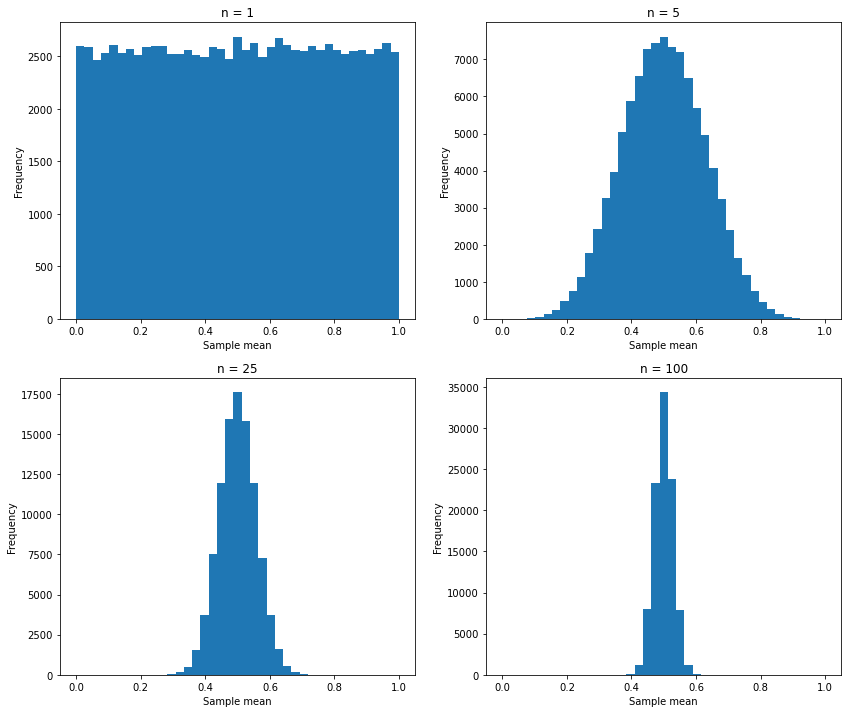
\includegraphics[scale=0.535]{part1/ch03-19d}
    \caption{Sampling distribution of $\overline{X}_n$ for different $n$.}
  \end{figure}

  Notice that as $n$ increases, the variance of the sampling distribution of
  $\overline{X}_n$ decreases, i.e.\ it becomes more narrow and sharply peaked
  around the true mean of the underlying distribution.
\end{ex}

% 20
\begin{ex}
  We begin by extending the definition of expectation to a random matrix, by
  defining the expected value of a random $m\times n$ matrix $X$ to be the
  $m\times n$ matrix whose $(i, j)$th entry is the expected value of $X_{i,j}$.

  Suppose that $X$ is a random matrix of dimension $m\times n$ with mean $\mu$,
  and let $A$ be a $p\times m$ matrix. Then
  \[
    \E{AX}_{i,j}
    =\E{\sum_{k=1}^m A_{i,k} X_{k,j}}
    =\sum_{i=1}^m A_{i,k}\E{X_{k,j}}
    =\sum_{i=1}^m A_{i,k}\mu_{k,j}
    =A\mu,
  \]
  and, likewise, if we let $B$ be an $n\times p$ matrix,
  \[
    \E{XB}_{i,j}
    =\E{\sum_{k=1}^n X_{i,k} B_{k,j}}
    =\sum_{i=1}^n \E{X_{i,k}}B_{k,j}
    =\sum_{i=1}^n \mu_{i,k}B_{k,j}
    =\mu B.
  \]

  The two claims about the expected value of $\E{a^TX}$ and $\E{AX}$ in Lemma
  3.21 are then special cases of this property for $X$ an $n\times 1$ random
  matrix.

  For the rest of the exercise we restrict $X$ to a random vector with mean
  $\mu$ and variance-covariance matrix $\Sigma$, and continue by noting that
  \begin{align*}
     & \E{(X-\mu)(X-\mu)^T}            \\
     & =\E{\begin{pmatrix}
        (X_1-\mu_1)^2          & (X_1-\mu_1)(X_2-\mu_2) & \cdots & (X_1-\mu_1)(X_n-\mu_n) \\
        (X_2-\mu_2)(X_1-\mu_1) & (X_2-\mu_2)^2          & \cdots & (X_2-\mu_2)(X_n-\mu_n) \\
        \vdots                 & \vdots                 & \ddots & \vdots                 \\
        (X_n-\mu_n)(X_1-\mu_1) & (X_n-\mu_n)(X_2-\mu_2) & \cdots & (X_n-\mu_n)^2          \\
      \end{pmatrix}} \\
     & =\begin{pmatrix}
      \var{X_1}      & \cov{X_1, X_2} & \cdots & \cov{X_1,X_n} \\
      \cov{X_2,X_1}  & \var{X_2}      & \cdots & \cov{X_2,X_n} \\
      \vdots         & \vdots         & \ddots & \vdots        \\
      \cov{X_n, X_1} & \cov{X_n, X_2} & \cdots & \var{X_n}     \\
    \end{pmatrix}     \\
     & =\var{X},
  \end{align*}
  and that therefore,
  \begin{align*}
    \var{AX}
     & =\E{(AX-A\mu)(AX-A\mu)^T} \\
     & =\E{A(X-\mu)(A(X-\mu))^T} \\
     & =\E{A(X-\mu)(X-\mu)^TA^T} \\
     & =A\E{(X-\mu)(X-\mu)^T}A^T \\
     & =A\Sigma A^T.
  \end{align*}

  This is the second claim about variances of random vectors in Lemma 3.21, but
  we conclude by noting that the first one is a special case of the second for
  matrices of the form $1\times n$.
\end{ex}

\begin{ex}
  Recall that by the rule of iterated expectations,
  \[
    \E{\cE{Y}{X}}=\E{Y},
  \]
  and therefore we have $\E{X}=\E{Y}$.

  Therefore,
  \begin{align*}
    \cov{X, Y}
     & =\E{XY} - \E{X}\E{Y} \\
  \end{align*}

  Likewise,
  \begin{align*}
    \E{XY}
     & =\E{\cE{XY}{X}}                     \\
     & =\int\! \cE{XY}{X=x} f_X(x) \,\d{x} \\
     & =\int\! \cE{Y}{X=x} xf_X(x) \,\d{x} \\
     & =\int\! x^2f_X(x) \,\d{x}           \\
     & =\E{X^2},
  \end{align*}
  and thus
  \begin{align*}
    \cov{X, Y}
     & =\E{XY} - \E{X}\E{Y} \\
     & =\E{X^2} - \E{X}^2   \\
     & = \var{X}.
  \end{align*}
\end{ex}

\begin{ex}
  \begin{enumerate}[(a)]
    \item[]
    \item No, since $\P{(Y, Z)=(1, 1)}=b-a$, while
          $\P{Y=1}=b$ and $\P{Z=1}=1-a$.
    \item We have
          \[
            \cE{Y}{Z=0}
            =\cP{Y=1}{Z=0}
            =\cP{Y=1}{X<a}
            =1,
          \]
          \[
            \cE{Y}{Z=1}
            =\cP{Y=1}{Z=1}
            =\cP{Y=1}{X>a}
            =\frac{b-a}{1-a}.
          \]
  \end{enumerate}
\end{ex}

\begin{ex}
  Suppose that $X\sim\text{Poisson}(\lambda)$. Then
  $f_X(x)=e^{-\lambda}\frac{\lambda^x}{x!}$ and thus
  \begin{align*}
    \psi_X(t)
     & =\E{e^{tX}}                                               \\
     & =\sum_{n=0}^\infty e^{tn}e^{-\lambda}\frac{\lambda^n}{n!} \\
     & =e^{-\lambda}\sum_{n=0}^\infty \frac{(\lambda e^t)^n}{n!} \\
     & =e^{\lambda(e^t-1)}.
  \end{align*}

  Suppose that $Y\sim N(\mu, \sigma^2)$. Then
  $f_Y=\frac{1}{\sqrt{2\pi\sigma^2}}
    \exp\left(-\frac{1}{2}\frac{(x-\mu)^2}{\sigma^2}\right)$,
  and therefore
  \begin{align*}
    \psi_Y(t)
     & =\E{e^{tY}}                                                  \\
     & =\int_{-\infty}^\infty\! e^{ty}\frac{1}{\sqrt{2\pi\sigma^2}}
    \exp\left(-\frac{1}{2}\frac{(y-\mu)^2}{\sigma^2}\right)\,\d{y}  \\
     & =\int_{-\infty}^\infty\! \frac{1}{\sqrt{2\pi\sigma^2}}
    \exp\left(-\frac{1}{2}\frac{(y-\mu)^2+ty\sigma^2}{\sigma^2}\right)\,\d{y}.
  \end{align*}
  However, since
  \begin{align*}
    -\frac{1}{2}(y-\mu)^2+ty\sigma^2
     & =-\frac{1}{2}(y^2-2y\mu+\mu^2-2ty\sigma^2)                                 \\
     & =-\frac{1}{2}(y^2-2y(\mu+t\sigma^2)+(\mu+t\sigma)^2-(\mu+t\sigma)^2+\mu^2) \\
     & =-\frac{1}{2}(y-\mu-t\sigma^2)^2+\frac{1}{2}((\mu+t\sigma^2)^2-\mu^2)      \\
     & =-\frac{1}{2}(y-\mu-t\sigma^2)^2+(t\mu\sigma^2+t^2\sigma^4/2),
  \end{align*}
  it follows that
  \begin{align*}
    \psi_Y(t)
     & =\exp(t\mu+t^2\sigma^2/2)\int_{-\infty}^\infty\! \frac{1}{\sqrt{2\pi\sigma^2}}
    \exp\left(-\frac{1}{2}\frac{(y-\mu-t\sigma^2)^2}{\sigma^2}\right)\,\d{y}          \\
     & =\exp(t\mu+t^2\sigma^2/2),
  \end{align*}
  since the integrand is the PDF for an $N(m+t\sigma^2, \sigma^2)$ distribution
  being integrated over its support.

  Suppose that $Z\sim\text{Gamma}(\alpha, \beta)$. Then
  \[
    f_Z(z)=\frac{1}{\beta^\alpha \Gamma(\alpha)}z^{\alpha-1}e^{-z/\beta}
  \]
  and so
  \begin{align*}
    \psi_Z(t)
     & =\E{e^{tZ}}                                                                                                                                   \\
     & =\int_{-\infty}^\infty e^{tz}\frac{1}{\beta^\alpha \Gamma(\alpha)}z^{\alpha-1}e^{-z/\beta}\,\d{z}                                             \\
     & =\int_{-\infty}^\infty \frac{1}{\beta^\alpha \Gamma(\alpha)}z^{\alpha-1}e^{-z(1/\beta-t)}\,\d{z}                                              \\
     & =\int_{-\infty}^\infty \frac{(1/\beta-t)^\alpha}{(1/\beta-t)^\alpha}\frac{1}{\beta^\alpha \Gamma(\alpha)}z^{\alpha-1}e^{-z(1/\beta-t)}\,\d{z} \\
     & =\frac{1}{(1/\beta-t)^\alpha\beta^\alpha}
    \int_{-\infty}^\infty \frac{1}{(1/\beta-t)^{-\alpha}\Gamma(\alpha)}z^{\alpha-1}e^{-z(1/\beta-t)}\,\d{z}                                          \\
     & =(1-\beta t)^{-\alpha},
  \end{align*}
  since the integrand is the PDF for a $\text{Gamma}(\alpha, (1/\beta-t)^{-1})$
  distribution integrated over its support.
\end{ex}

\begin{ex}
  Note that $f_{X_i}(x)=\frac{1}{\beta} e^{-x/\beta}$ and that therefore
  \begin{align*}
    \psi_{X_i}(t)
     & =\E{e^{tX_i}}                                                                                           \\
     & =\int_{0}^\infty e^{tx}\frac{1}{\beta} e^{-x/\beta}\,\d{x}                                              \\
     & =\int_0^\infty\!\frac{1}{\beta}\exp\left(-x/(\beta/(1-\beta t))\right)\,\d{t}                           \\
     & =(1-\beta t)^{-1}\int_0^\infty\! \frac{1-\beta t}{\beta} \exp\left(-x/(\beta/(1-\beta t))\right)\,\d{t} \\
     & =(1-\beta t)^{-1}
  \end{align*}
  since the integrand is the PDF for an exponential distribution integrated over
  its support.

  Let $Y=\sum_{i=1}^n X_i$. Then
  \[
    \psi_Y(t)
    =\prod_{i=1}^n \psi_{X_i}(t)
    =\left(1-\beta t\right)^{-n},
  \]
  which by the previous problem is the MGF of a $\text{Gamma}(n,\beta)$
  distribution.
\end{ex}
